\subsubsection{Design of a PD based CO-Trainer}

Proportional integral derivative (PID) shown in \cref{eq:pid} can be applied for making a simple aviation helper in piloting the quadcopter. For basic flight stabilization, a simple PD action can provide satisfactory performance shown in \cref{fig:pd}.

\begin{figure}
    \caption{Comparison of PID and PD}\label{fig:pd}
    \centering
    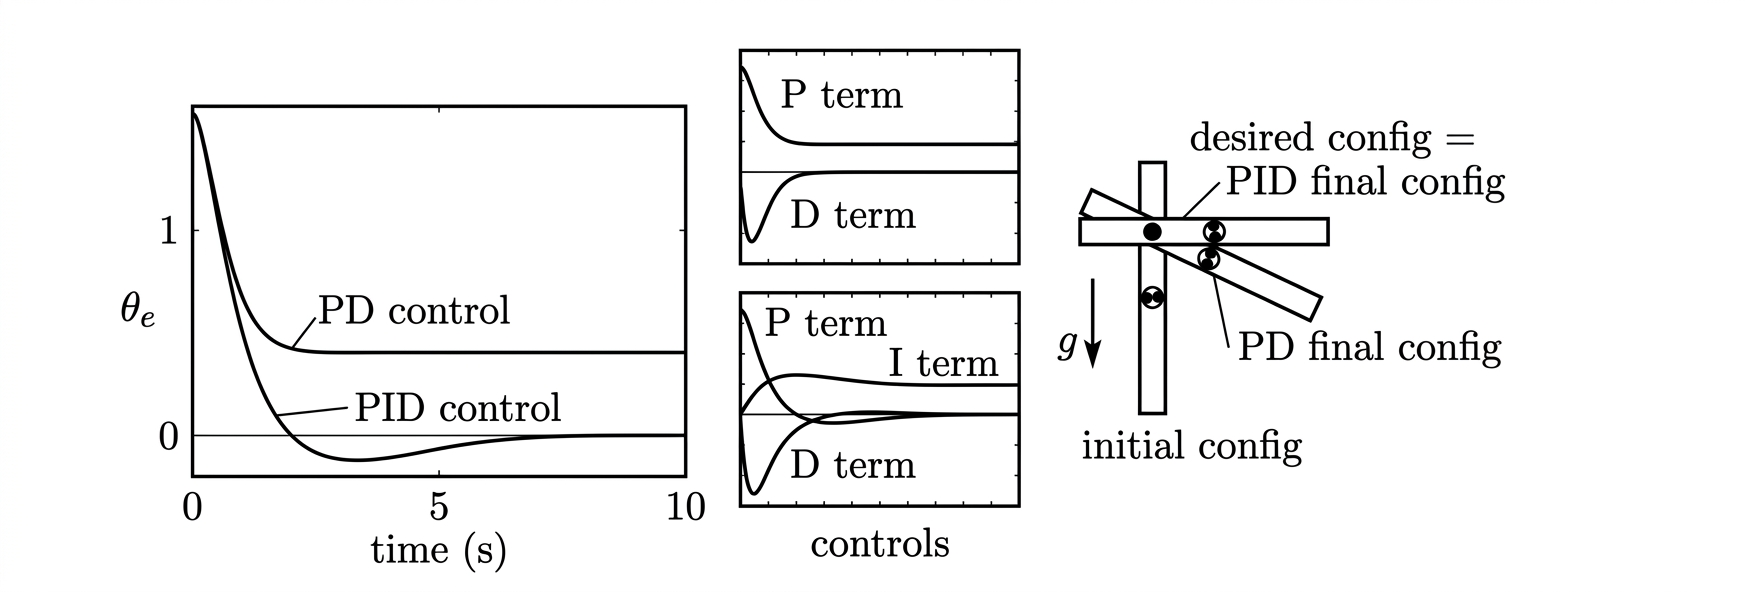
\includegraphics[width=0.8\linewidth]{img/pid.png}
\end{figure}

For attitude control, The error between the target orientation $q_{\text{target}}$ and the current body orientation $q_{\text{body}}$ is defined as \cref{eq:attitude}.

\begin{equation}\label{eq:attitude}
    \Delta q = q_{\text{target}} \cdot q_{\text{body}}^{-1}
\end{equation}

Using Unity's ToAngleAxis method, this relative rotation is converted into an angle $\phi$ and an axis $\mathbf{n}$. The error vector $\mathbf{e}$ is then $\mathbf{e} = \phi \cdot \mathbf{n}$.

The controller applies a PD loop (Proportional-Derivative) to generate corrective torque shown in \cref{eq:pdt}.

\begin{equation}\label{eq:pdt}
    \boldsymbol{\tau}_{\text{world}} = K_p \cdot \mathbf{e} + K_d \cdot \frac{\mathbf{e} - \mathbf{e}_{k-1}}{\Delta t}
\end{equation}

The world-space torque is transformed into the body frame ($R_{\text{wb}}$) for the physics simulation: $\boldsymbol{\tau}_{\text{body}} = R_{\text{wb}} \cdot \boldsymbol{\tau}_{\text{world}}$

The controller should be able to pilot the quadcopter in a closed-loop mission. The system employs a cascaded control scheme where the Outer Loop (Position) provides setpoints for the Inner Loop (Attitude/Velocity).

The Inner Loop features controllers that yield the required rolling and pitching moments $\tau_x$ and $\tau_y$ to regulate horizontal movement. The Inner Loop block requires the current quadcopter attitude as well as reference signals for roll and pitch to obtain its output \parencite{paredes2021quadcopter}; The Outer Loop, which features controllers that yield the required thrust differential and yawing moments as well as the desired reference signals.

During takeoff, the controller focuses exclusively on vertical error ($e_y$). The vertical force $force_Y$ is mapped to a normalized throttle value ($T$) shown in \cref{eq:mappingt}.

Following a path requires a look-ahead method. Given current position $\mathbf{p}$ and look-ahead target $\mathbf{t}$ on the path, the position error is defined as: $e_x = t_x - p_x,\quad e_y = t_y - p_y,\quad e_z = t_z - p_z$. 

The Outer Loop converts this error into a desired velocity in the world axis as shown in \cref{eq:outerLoop}.

\begin{equation}\label{eq:outerLoop}
    v_{x,\text{des}} = \text{PD}_X(e_x),\quad v_{z,\text{des}} = \text{PD}_Z(e_z)
\end{equation}

To translate these into drone-relative commands (Pitch/Roll), the world velocity is projected onto the drone's Heading Axis: (1) Forward Basis: $\hat{\mathbf{f}} = R_y(\psi)\,\hat{\mathbf{z}}_{\text{forward}}$; (2) Right Basis: $\hat{\mathbf{r}} = R_y(\psi)\,\hat{\mathbf{x}}_{\text{right}}$; The projections shown as \cref{eq:projection}. Where $e_{v,\parallel}$ is the longitudinal velocity error,  $e_{v,\perp}$ is the lateral velocity error.

\begin{equation}\label{eq:projection}
    v^{\parallel}_{\text{des}} = \mathbf{v}_{H,\text{des}}\cdot\hat{\mathbf{f}}, \quad v^{\perp}_{\text{des}} = \mathbf{v}_{H,\text{des}}\cdot\hat{\mathbf{r}}
\end{equation}

The Inner Loop then calculates the error between desired and actual velocity to produce stick inputs. Pitch (Right Vertical): Based on $e_{v,\parallel}$; Roll (Right Horizontal): Based on $e_{v,\perp}$.

The target yaw speed $\psi_{\text{target}} = \operatorname{atan2}(v_x,\,v_z)$, the yaw error is  $e_\psi = \text{DeltaAngle}(\psi, \psi_{\text{target}})$, so mapped to joystick movement is $u_{\text{yaw}} = \text{PID}_{\text{yaw}}(e_\psi)$. The other axis are the same methods.